%\begin{figure}[hbt]
%  \centering
%  \label{fig:}
%  \subfigure[CAP]{
%    \includegraphics[width=0.4\textwidth]{}
%  }
%  \caption{}
%\end{figure}

~\vfill

\begin{figure}[hbt]
  \centering
  \label{fig:convolution}
  \subfigure[Original]{
    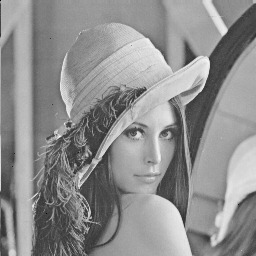
\includegraphics[width=0.3\textwidth]{../images/lenna}
  }
  \subfigure[15x15 Frequency Domain]{
    \includegraphics[width=0.3\textwidth]{../images/lenna_15_freq}
  }
  \subfigure[15x15 Spacial Domain]{
    \includegraphics[width=0.3\textwidth]{../images/lenna_15_space}
  } \\
  \hspace{0.317\textwidth}
  \subfigure[7x7 Frequency Domain]{
    \includegraphics[width=0.3\textwidth]{../images/lenna_7_freq}
  }
  \subfigure[7x7 Spacial Domain]{
    \includegraphics[width=0.3\textwidth]{../images/lenna_7_space}
  } \\
  \subfigure[Original]{
    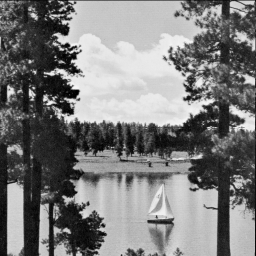
\includegraphics[width=0.3\textwidth]{../images/boat}
  }
  \subfigure[15x15 Frequency Domain]{
    \includegraphics[width=0.3\textwidth]{../images/boat_15_freq}
  }
  \subfigure[15x15 Spacial Domain]{
    \includegraphics[width=0.3\textwidth]{../images/boat_15_space}
  } \\
  \hspace{0.317\textwidth}
  \subfigure[7x7 Frequency Domain]{
    \includegraphics[width=0.3\textwidth]{../images/boat_7_freq}
  }
  \subfigure[7x7 Spacial Domain]{
    \includegraphics[width=0.3\textwidth]{../images/boat_7_space}
  } \\
  \caption{Two images convolved with 15x15 and 7x7 Gaussian.  Compairison of convolution
    using the convolution theorem and convolution in the spacial domain.}
\end{figure}

\newcolumntype{T}{>{\centering\arraybackslash} m{0.10\textwidth} }
\newcolumntype{S}{>{\centering\arraybackslash} m{0.135\textwidth} }
\begin{tabular}{ T S @{} S @{} S @{} S @{} S @{} S }
  \centering
  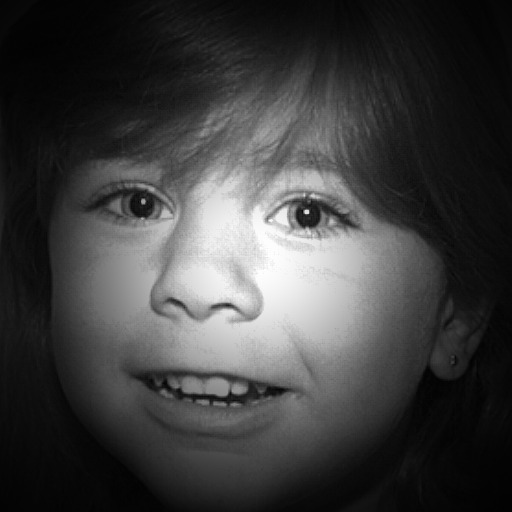
\includegraphics[width=0.1\textwidth]{../images/girl}
  & $\gamma_L=0.2$ & $\gamma_L=0.3$ & $\gamma_L=0.4$ & $\gamma_L=0.5$ & $\gamma_L=0.6$ & $\gamma_L=0.7$ \\
  $\gamma_H=1.2$
  & 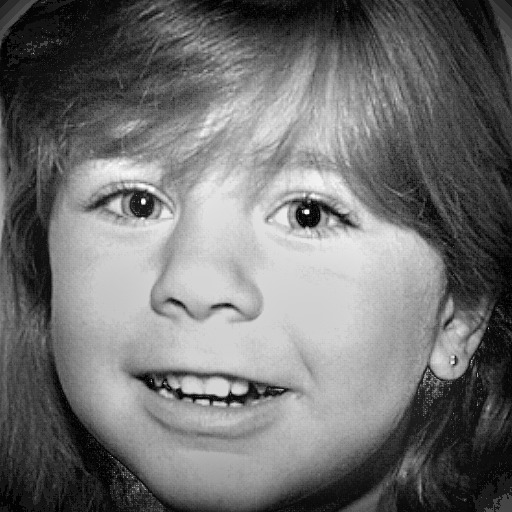
\includegraphics[width=0.135\textwidth]{../images/girl_2_12}
  & 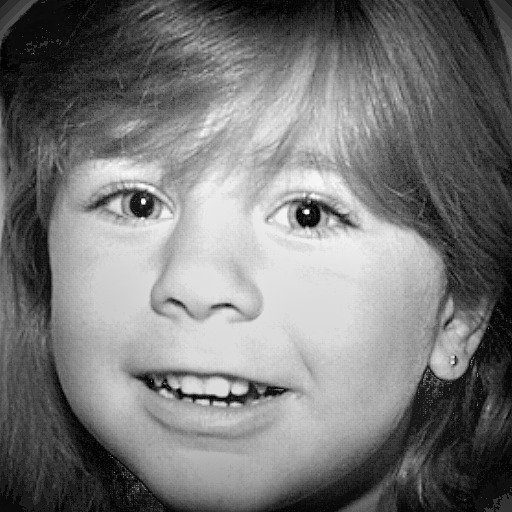
\includegraphics[width=0.135\textwidth]{../images/girl_3_12}
  & 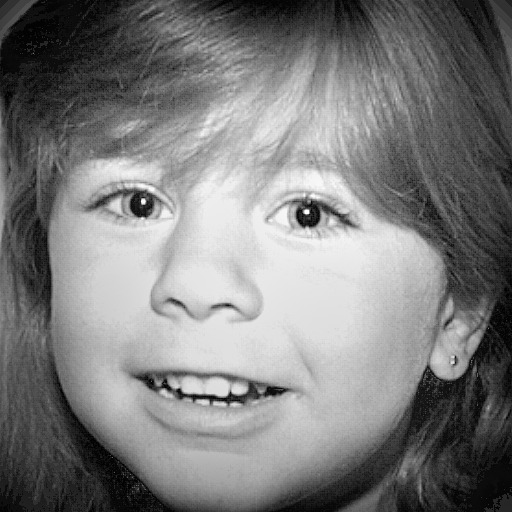
\includegraphics[width=0.135\textwidth]{../images/girl_4_12}
  & 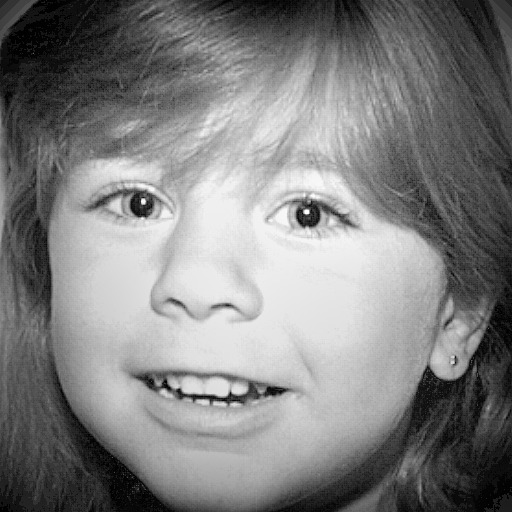
\includegraphics[width=0.135\textwidth]{../images/girl_5_12}
  & 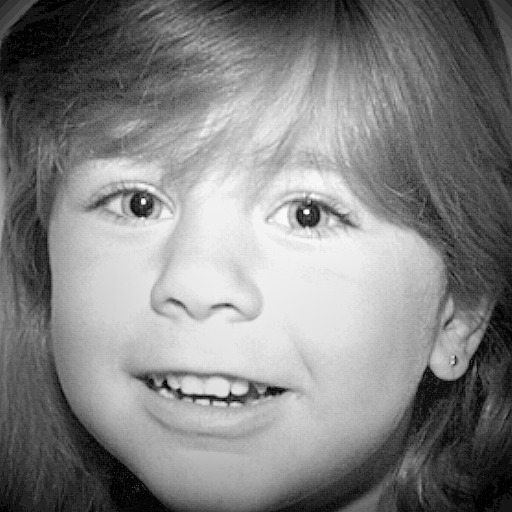
\includegraphics[width=0.135\textwidth]{../images/girl_6_12}
  & 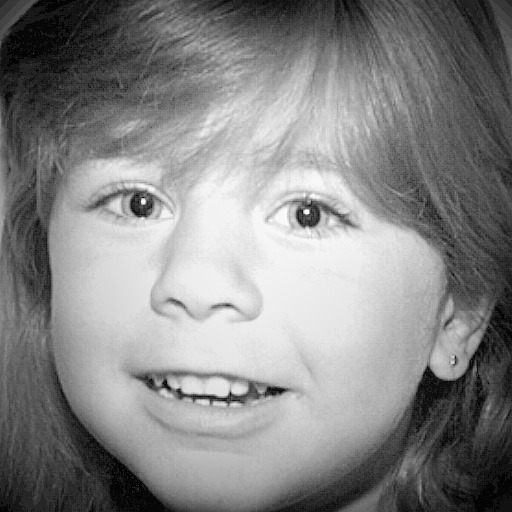
\includegraphics[width=0.135\textwidth]{../images/girl_7_12} \\ [-4pt]
  $\gamma_H=1.3$
  & 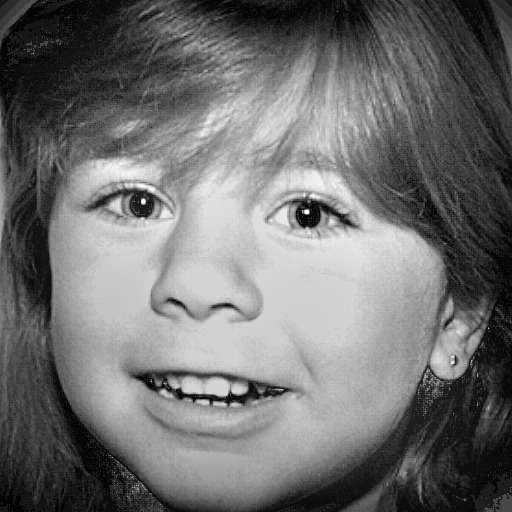
\includegraphics[width=0.135\textwidth]{../images/girl_2_13}
  & 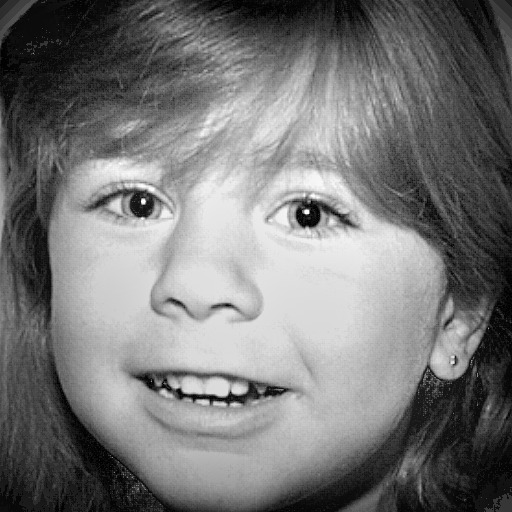
\includegraphics[width=0.135\textwidth]{../images/girl_3_13}
  & 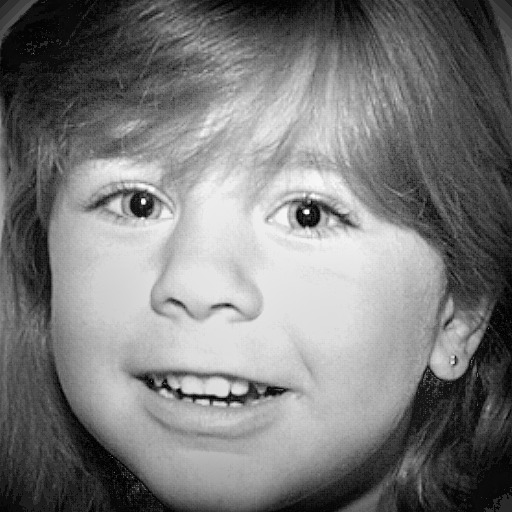
\includegraphics[width=0.135\textwidth]{../images/girl_4_13}
  & 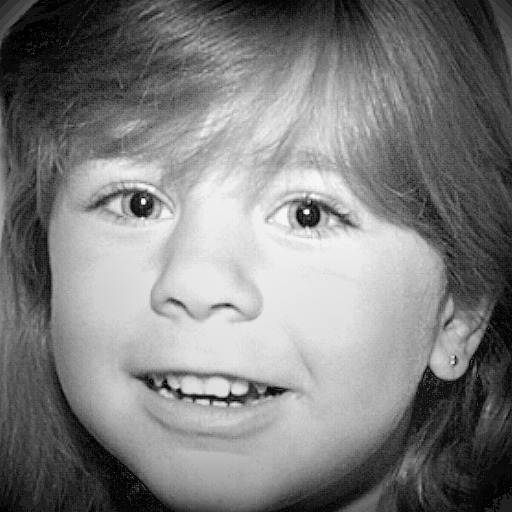
\includegraphics[width=0.135\textwidth]{../images/girl_5_13}
  & 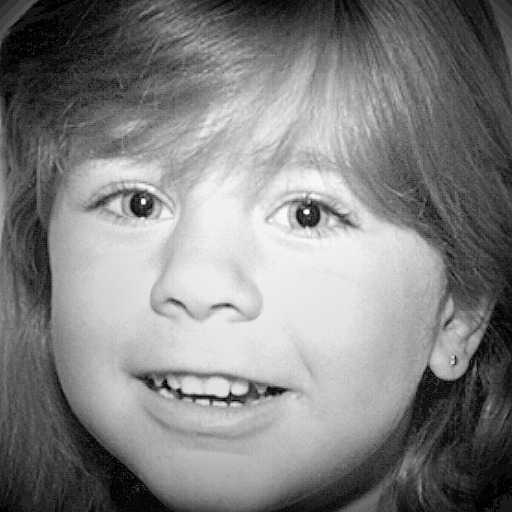
\includegraphics[width=0.135\textwidth]{../images/girl_6_13}
  & 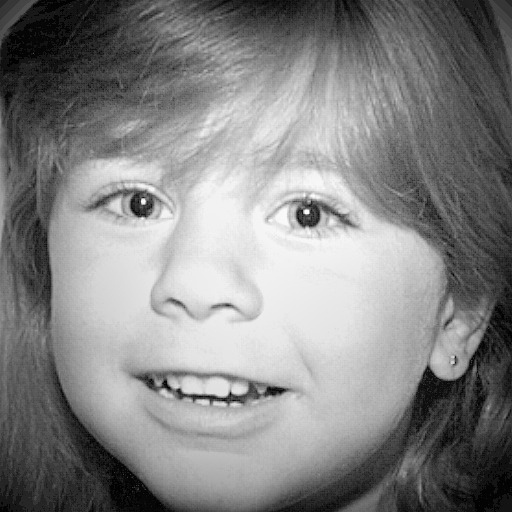
\includegraphics[width=0.135\textwidth]{../images/girl_7_13} \\ [-4pt]
  $\gamma_H=1.4$
  & 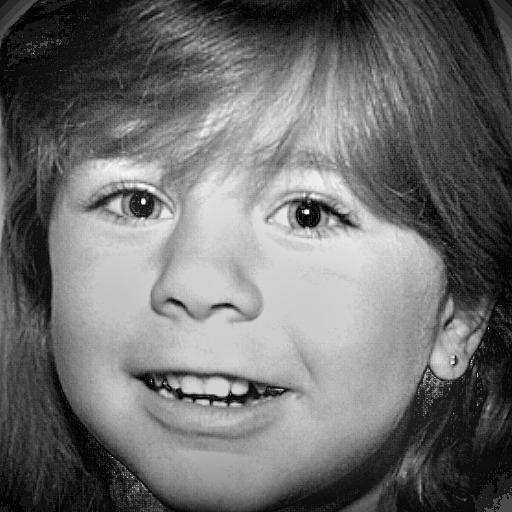
\includegraphics[width=0.135\textwidth]{../images/girl_2_14}
  & 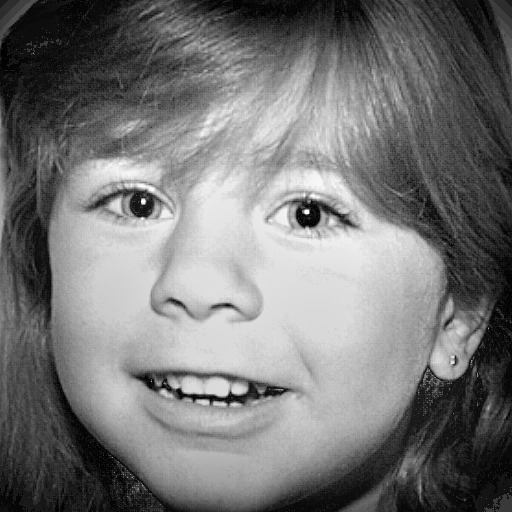
\includegraphics[width=0.135\textwidth]{../images/girl_3_14}
  & 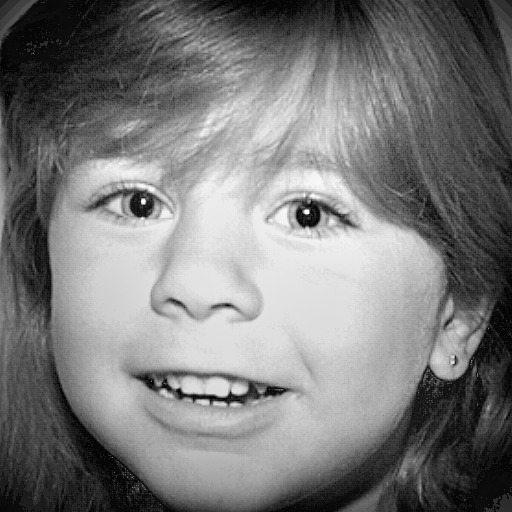
\includegraphics[width=0.135\textwidth]{../images/girl_4_14}
  & 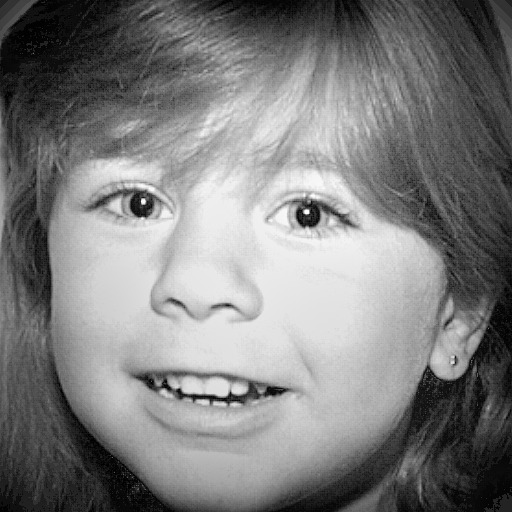
\includegraphics[width=0.135\textwidth]{../images/girl_5_14}
  & 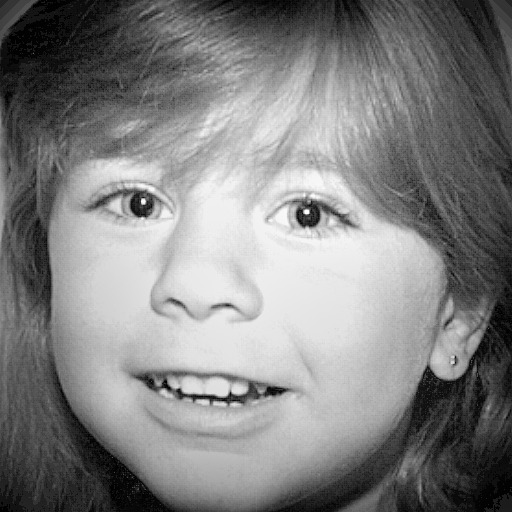
\includegraphics[width=0.135\textwidth]{../images/girl_6_14}
  & 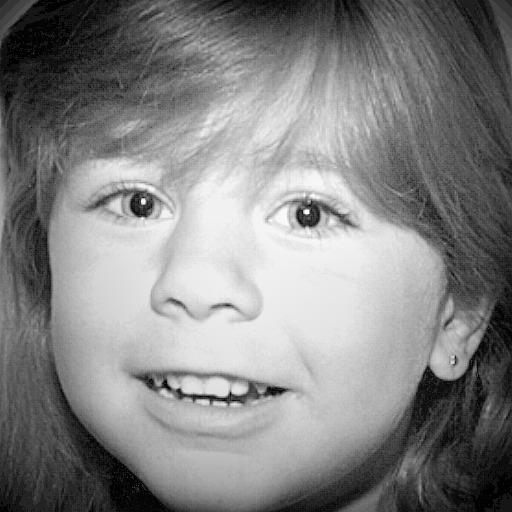
\includegraphics[width=0.135\textwidth]{../images/girl_7_14} \\ [-4pt]
  $\gamma_H=1.5$
  & 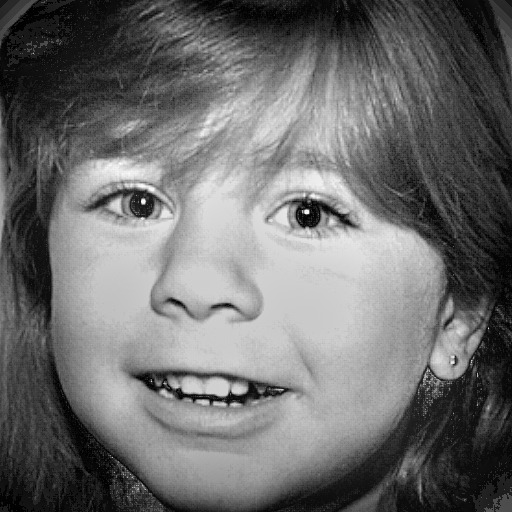
\includegraphics[width=0.135\textwidth]{../images/girl_2_15}
  & 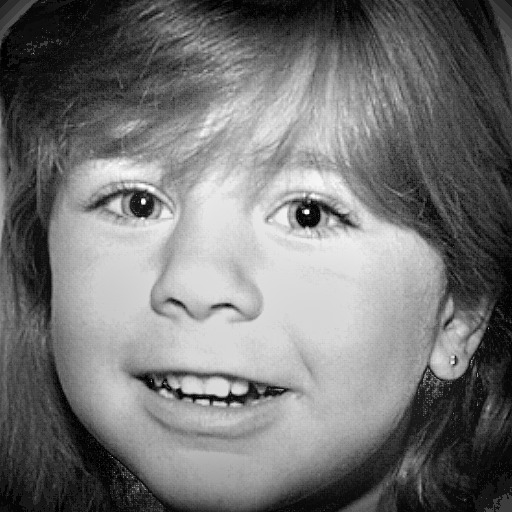
\includegraphics[width=0.135\textwidth]{../images/girl_3_15}
  & 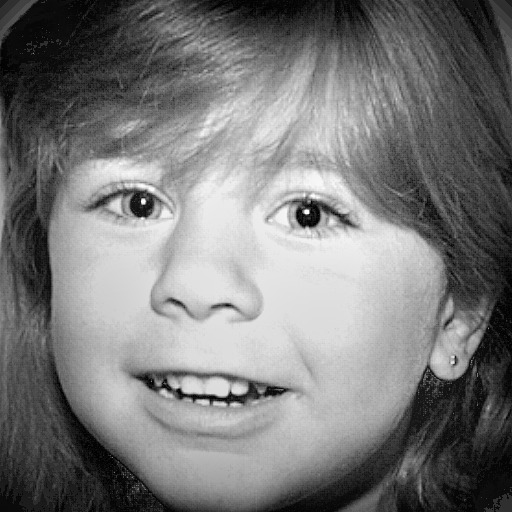
\includegraphics[width=0.135\textwidth]{../images/girl_4_15}
  & 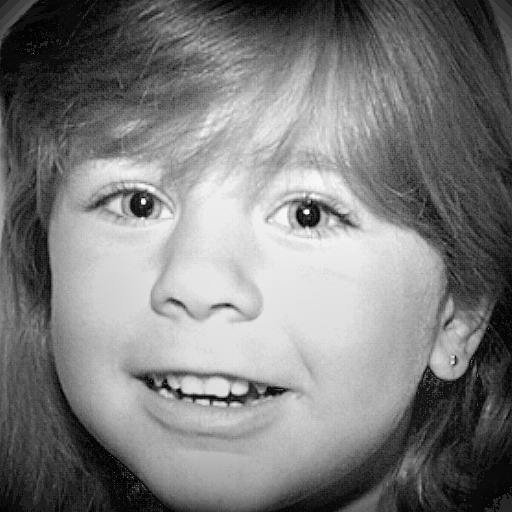
\includegraphics[width=0.135\textwidth]{../images/girl_5_15}
  & 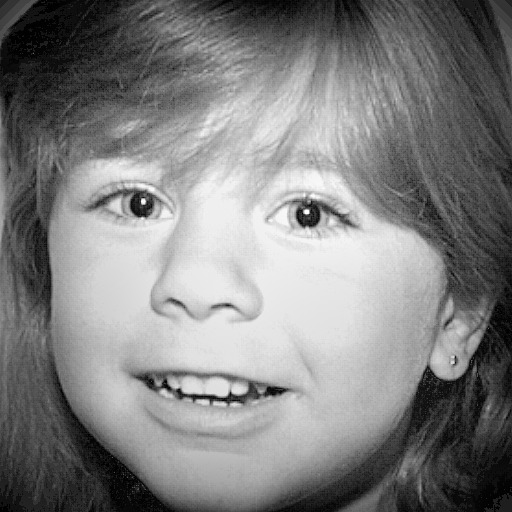
\includegraphics[width=0.135\textwidth]{../images/girl_6_15}
  & 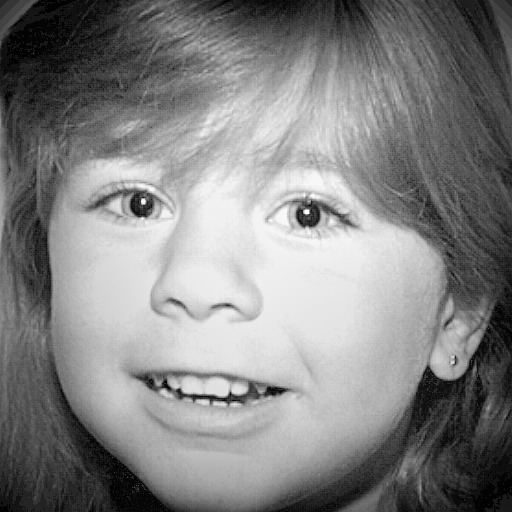
\includegraphics[width=0.135\textwidth]{../images/girl_7_15} \\ [-4pt]
  $\gamma_H=1.6$
  & 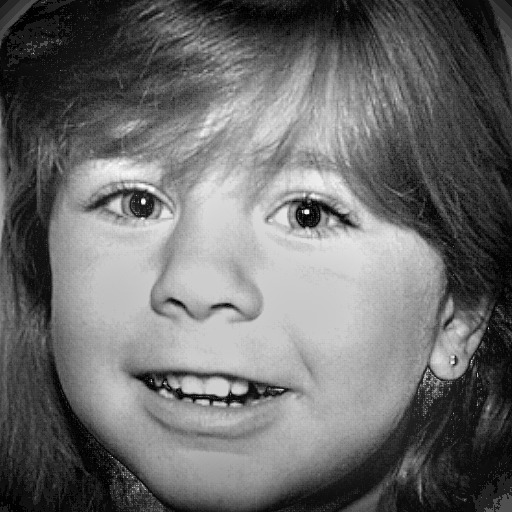
\includegraphics[width=0.135\textwidth]{../images/girl_2_16}
  & 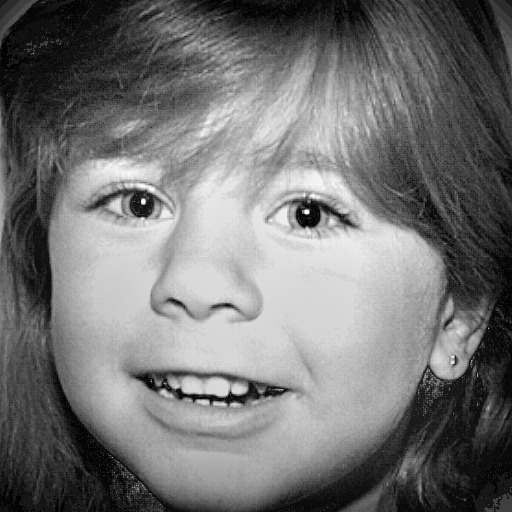
\includegraphics[width=0.135\textwidth]{../images/girl_3_16}
  & 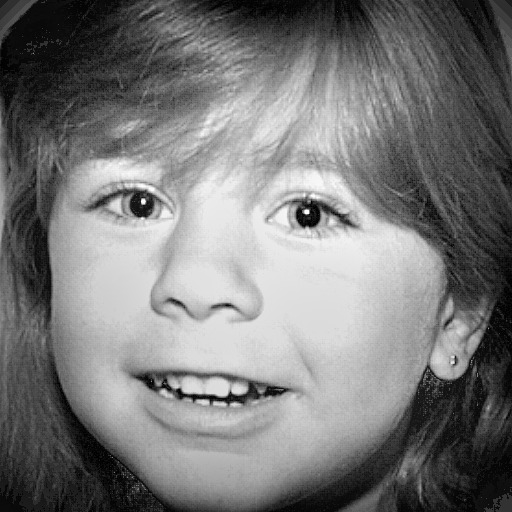
\includegraphics[width=0.135\textwidth]{../images/girl_4_16}
  & 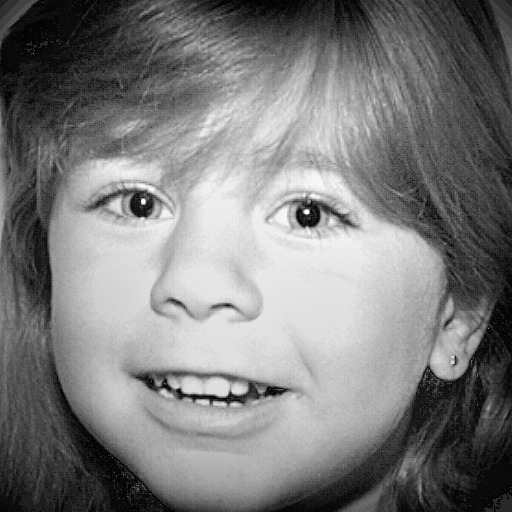
\includegraphics[width=0.135\textwidth]{../images/girl_5_16}
  & 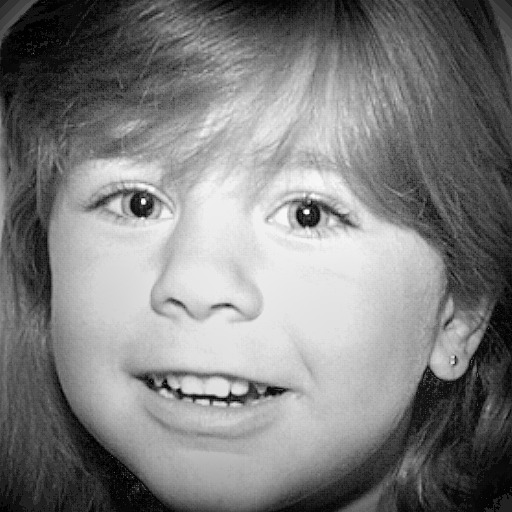
\includegraphics[width=0.135\textwidth]{../images/girl_6_16}
  & 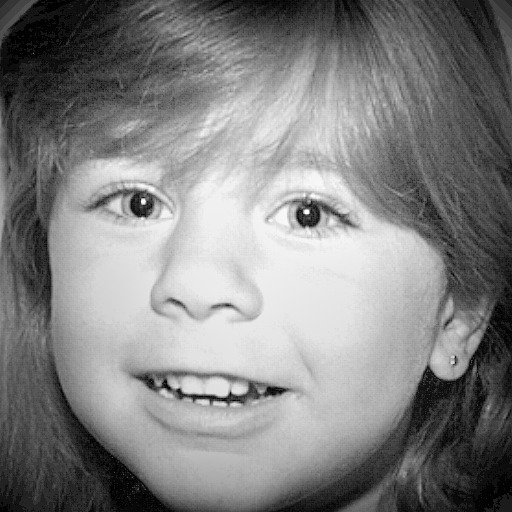
\includegraphics[width=0.135\textwidth]{../images/girl_7_16} \\ [-4pt]
  $\gamma_H=1.7$
  & 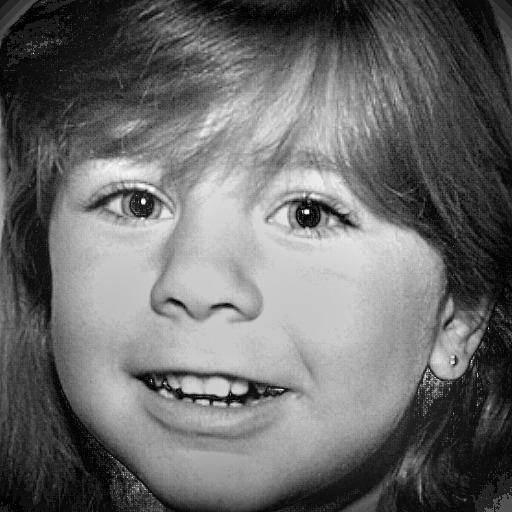
\includegraphics[width=0.135\textwidth]{../images/girl_2_17}
  & 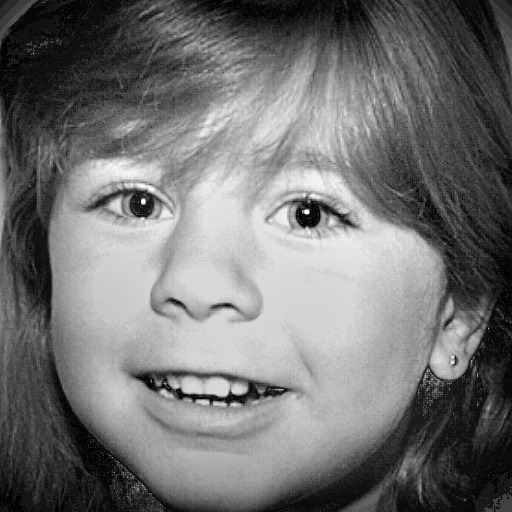
\includegraphics[width=0.135\textwidth]{../images/girl_3_17}
  & 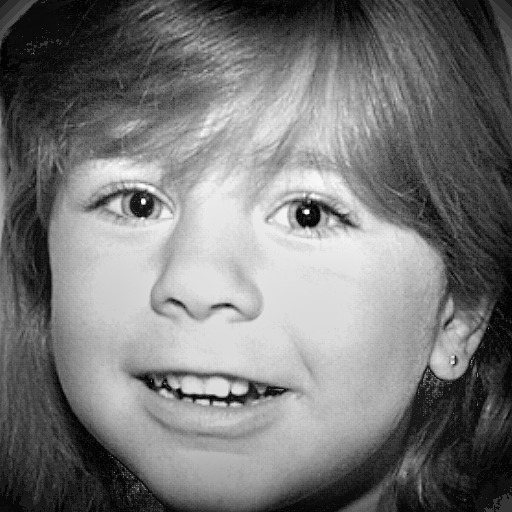
\includegraphics[width=0.135\textwidth]{../images/girl_4_17}
  & 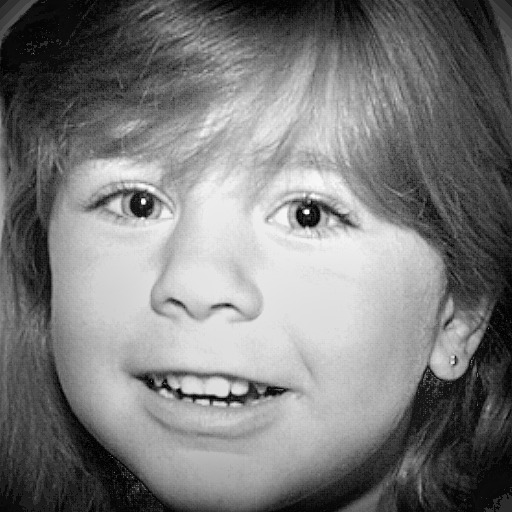
\includegraphics[width=0.135\textwidth]{../images/girl_5_17}
  & 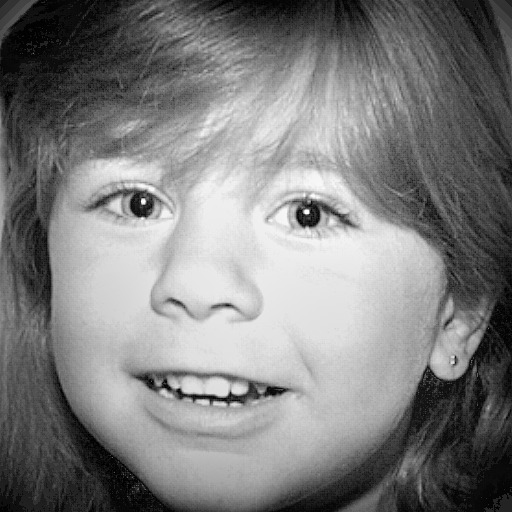
\includegraphics[width=0.135\textwidth]{../images/girl_6_17}
  & 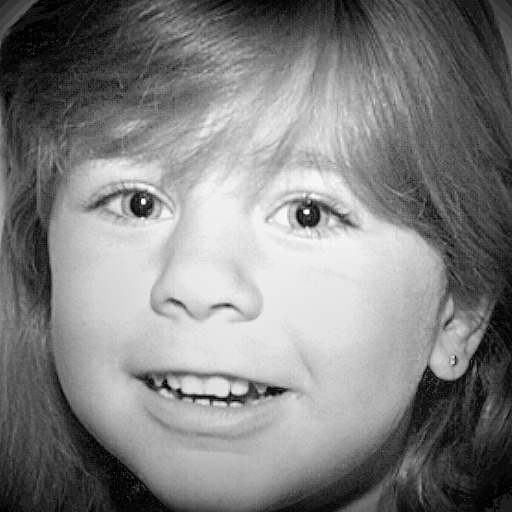
\includegraphics[width=0.135\textwidth]{../images/girl_7_17} \\ [-4pt]

  
\end{tabular}
\vfill
